\documentclass[conference]{IEEEtran}
\IEEEoverridecommandlockouts
\usepackage{amsmath,amssymb}
\usepackage{graphicx}
\usepackage{booktabs}
\usepackage{array}
\usepackage{float}
\usepackage{algorithm}
\usepackage{algorithmic}
\usepackage{cite}
\usepackage{url}
\usepackage{xcolor}
\usepackage{microtype}
\usepackage[hidelinks]{hyperref}
\graphicspath{{figures/}}
\setlength{\textfloatsep}{5pt plus 1pt minus 1pt}
\setlength{\floatsep}{4pt plus 1pt minus 1pt}
\setlength{\intextsep}{4pt plus 1pt minus 1pt}
\setlength{\abovecaptionskip}{3pt}
\setlength{\belowcaptionskip}{0pt}

\title{CREATE: Training-Evidence-Guided Reward Repair for Reinforcement Learning}

\author{\IEEEauthorblockN{Anonymous Authors}
\IEEEauthorblockA{Anonymous Submission}}

\begin{document}
\maketitle

\begin{abstract}
Evaluating a language-model-generated reward requires a complete
reinforcement-learning run, yet most reward-search methods use that run only
to rank or replace candidates. We introduce
\textbf{CREATE}, a \textbf{C}losed-loop \textbf{R}eward \textbf{E}diting
\textbf{A}gent with \textbf{T}raining \textbf{E}vidence, which treats each run
as an observation for repairing the active reward lineage. CREATE combines
native-task outcomes with component activation and magnitude statistics,
stores diagnoses and edit outcomes in persistent memory, and applies one
severity-gated intervention while a best archive protects the returned
solution. Experiments on discrete and continuous Gymnasium control tasks show
that CREATE reliably repairs initially unsuccessful rewards and that the
selected rewards remain effective on independent test seeds. Mechanism
ablations show that component-level evidence and single-target editing are
complementary: feedback must localize the failure, and the action must preserve
attribution to one change. Repair traces reveal two distinct routes to
improvement---L1 scale correction for a sound reward form and L2 structural
refactoring for unreachable or exploitable components. These results support
closed-loop diagnosis as a more informative use of policy-training outcomes
than repeated prompting alone.
\end{abstract}

\begin{IEEEkeywords}
reinforcement learning, reward design, large language models, language agents,
learning-based control
\end{IEEEkeywords}

\section{Introduction}
Reward design translates a task objective into the signal optimized by a
reinforcement-learning (RL) policy. In practice, it is a debugging loop: write
a reward, train a policy, inspect the behavior, and revise the reward. Policy
training is the expensive step, but its output contains far more than one
score. Component activations reveal unreachable bonuses, magnitude shares
expose dominating terms, and episode outcomes distinguish task failure from
reward exploitation. These measurements complement the standard return-based
view of RL~\cite{sutton2018rl}. Our formulation is motivated by
reward-shaping failures~\cite{ng1999policy} and the broader problem of reward
misspecification~\cite{hadfield2017inverse}.

Code-capable LLMs can translate task descriptions into executable dense
rewards~\cite{language2rewards}. Text2Reward emphasizes interpretable reward
programs~\cite{text2reward}, while Eureka uses evolutionary search with reward
reflection~\cite{eureka}. Later systems add dynamic trajectory
feedback~\cite{card}, preference feedback~\cite{revolve}, or agentic tree
search~\cite{rfagent}. These
approaches mainly ask which candidate should survive. We ask a complementary
question: \emph{what should the next reward change, given everything observed
while training the current one?}

We answer with \textbf{CREATE}, a \emph{Closed-loop Reward Editing Agent with
Training Evidence}. CREATE turns each completed policy-training run into an
observation, diagnoses one primary failure, and applies one bounded action to
the active reward lineage. Persistent memory conditions the diagnosis; the
trainer and environment execute the selected edit; and a best archive protects
earlier solutions when a later experiment regresses. Thus, ``agent'' denotes a
closed observation--memory--action--transition loop, not merely repeated LLM
calls.

Taken together, the paper reframes reward design as repair at the
policy-training timescale rather than repeated one-shot generation. The
resulting formulation separates the generated reward used for learning from
the native objective used for evaluation, equips the diagnostic agent with
severity-gated and component-bounded actions, and tests the complete loop with
budget-matched search, mechanism ablations, independent test episodes, and
evidence-level case analysis on two control benchmarks.

\section{Related Work}
\subsection{Reward Specification and Misspecification}
Reward shaping can accelerate learning, but only restricted transformations
preserve the optimal policy~\cite{ng1999policy}. Inverse reward design instead
treats the specified objective as evidence about an imperfect designer and
reasons about the intended objective~\cite{hadfield2017inverse}. Both lines
motivate separating the signal optimized during training from the objective
used to judge behavior. CREATE operationalizes that separation: the policy
optimizes generated reward code, while an untouched native evaluator supplies
the agent's external outcome signal.

\subsection{LLM-Based Reward Synthesis and Search}
Language to Rewards maps task descriptions to dense robot reward
programs~\cite{language2rewards}, and Text2Reward emphasizes executable and
interpretable reward code~\cite{text2reward}. Eureka couples code generation
with evolutionary search and reward reflection~\cite{eureka}. CARD augments
revision with dynamic trajectory feedback~\cite{card}; REvolve introduces
human preference feedback~\cite{revolve}; and RF-Agent organizes reward
construction as language-agent tree search~\cite{rfagent}. These systems show
that feedback improves generation, but candidate selection and broad
regeneration can obscure which reward mechanism caused the next outcome.
CREATE is deliberately depth-oriented: it preserves one lineage, identifies
one primary failure, and spends the next expensive training run on a bounded,
auditable intervention.

\begin{figure*}[t]
\centering
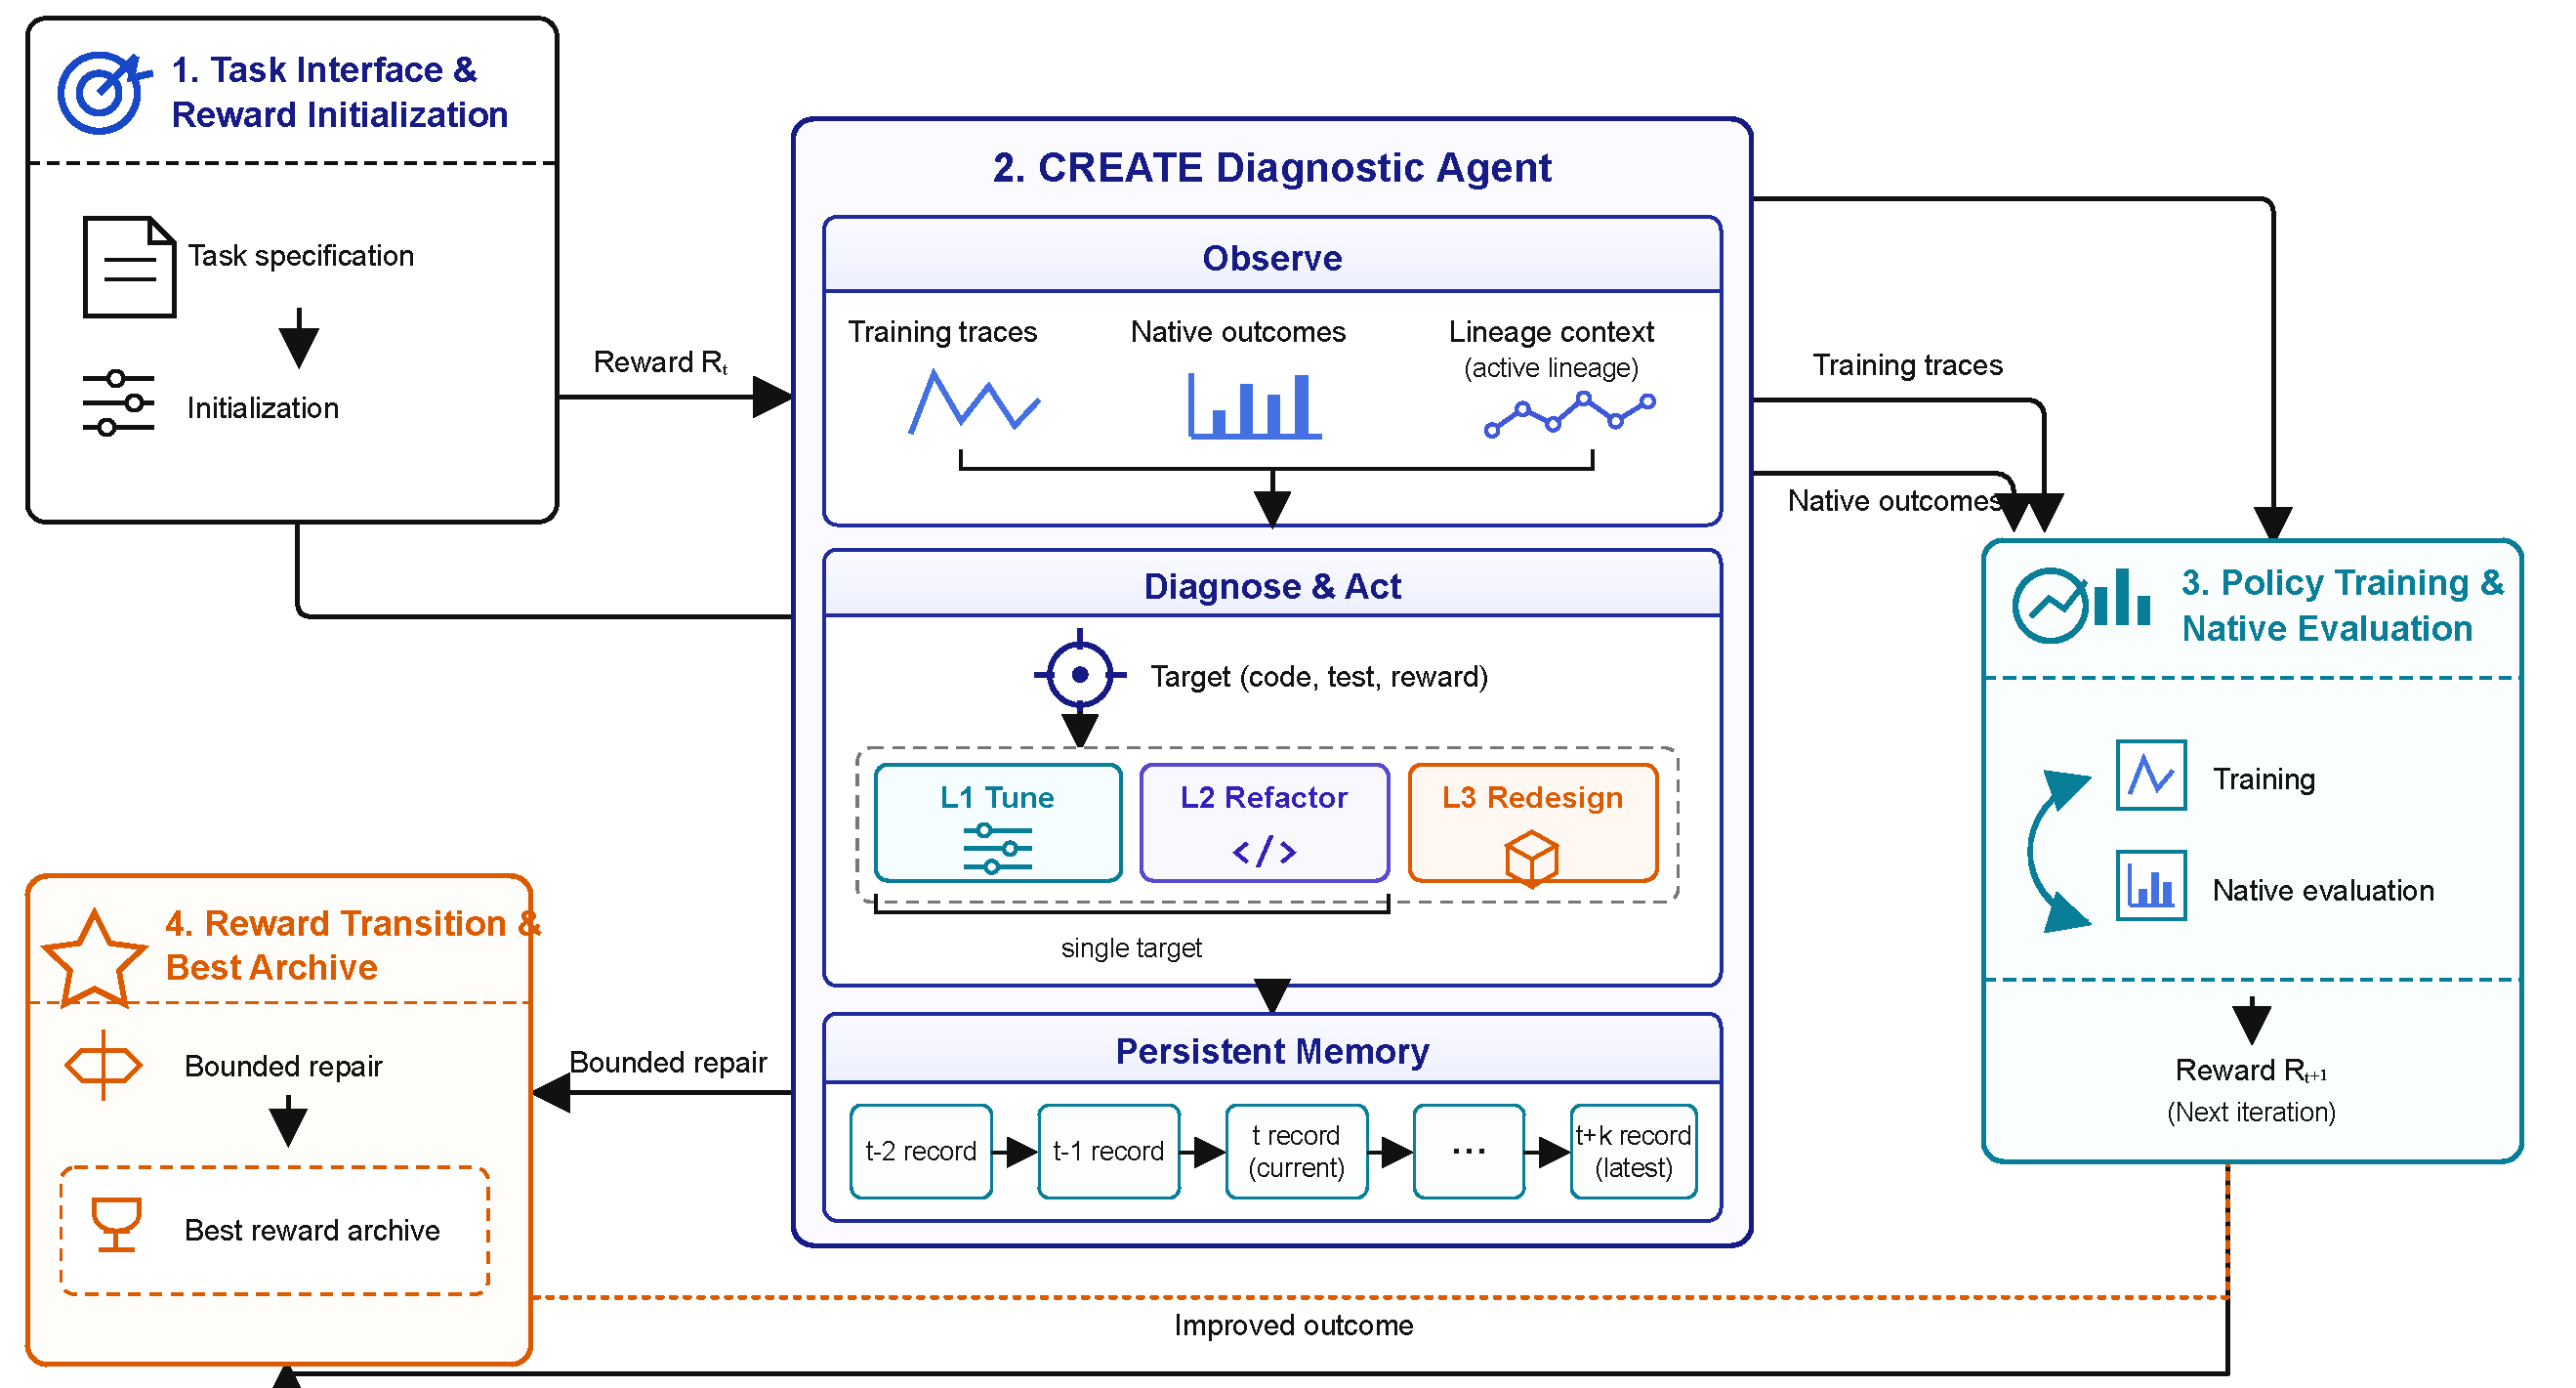
\includegraphics[width=0.98\textwidth]{framework.pdf}
\caption{CREATE's closed reward-repair loop. Task initialization yields
$R_0$. PPO training and native evaluation return training traces and $J_t$.
The agent diagnoses one failure, applies an L1/L2/L3 single-target repair,
records the transition in persistent memory, validates $R_{t+1}$, and updates
the best archive only when native performance improves.}
\label{fig:framework}
\end{figure*}

\subsection{Feedback-Driven Language Agents}
ReAct establishes the observation--reasoning--action pattern by interleaving
verbal reasoning with actions that obtain external feedback~\cite{react}.
Reflexion shows how stored verbal feedback can alter later decisions without
updating model weights~\cite{reflexion}, while Voyager combines iterative
environment feedback, self-verification, and a persistent skill
library~\cite{voyager}. CREATE adopts these functional agent properties at a
different timescale: one action edits a reward program, and one environment
transition is a complete policy-training and native-evaluation run. Its memory
stores hypotheses, edits, predictions, and outcomes rather than only a chat
history.

\subsection{Diagnostic Reward Refinement}
Recent diagnostic-driven reward refinement casts reward failure as debugging
and emphasizes that useful diagnostic vocabularies depend on task
structure~\cite{wang2026diagnostic}. CREATE complements that direction with a
fully specified control interface: component-level measurements localize a
failure; severity gates the L1/L2/L3 action space; program checks reject
invalid edits before training; and a best-so-far archive protects the returned
solution. The distinguishing claim is therefore not that an LLM can revise a
reward, but that training evidence, bounded action, persistent state, and
external transition jointly form an auditable reward-repair agent.

\section{CREATE}
\subsection{Task Interface and Agent State}
CREATE acts once per completed reward evaluation, not once per environment
step. At iteration $t$, the policy learner and native evaluator produce an
observation; the reward-repair agent then chooses the next reward program.
Table~\ref{tab:agent} summarizes the state carried across this decision cycle.

\begin{table}[t]
\caption{CREATE reward-repair decision interface.}
\label{tab:agent}
\centering
\scriptsize
\setlength{\tabcolsep}{3.1pt}
\begin{tabular}{p{0.16\columnwidth}p{0.39\columnwidth}p{0.35\columnwidth}}
\toprule
State element & Implementation & Role in the decision cycle \\
\midrule
Observation & Native outcome plus reward-component statistics & Localize the
current failure \\
Memory & Prior rewards, diagnoses, edits, and outcomes & Condition the next
decision on the lineage \\
Action & L1 tune, L2 refactor, or exceptional L3 redesign & Restrict the change
being tested \\
Transition & Execute the edited reward through a new policy training run &
Obtain external feedback \\
Archive & Best reward--policy pair seen so far & Return the incumbent, not the
last edit \\
\bottomrule
\end{tabular}
\end{table}

Let the agent state be
\begin{equation}
x_t=(R_t,M_t,A_t^\star),
\label{eq:state}
\end{equation}
where $R_t$ is the active reward program, $M_t$ is its lineage memory, and
$A_t^\star$ is the best reward--policy pair observed so far. Policy training
uses the generated reward,
\begin{equation}
(\pi_t,T_t)=\operatorname{Train}(\mathcal{E},R_t;B),
\label{eq:train}
\end{equation}
but policy quality is measured only with the untouched native objective:
\begin{equation}
J_t=\frac{1}{N}\sum_{i=1}^{N}\sum_{k=0}^{H_i-1}
r_{\rm env}(s_k^i,a_k^i,s_{k+1}^i).
\label{eq:native}
\end{equation}
This prevents a generated reward from declaring its own success. Each
completed candidate consumes the same fixed interaction budget $B$; after
$n$ evaluations the primary cost is therefore $C(n)=nB$.

\subsection{Training-Evidence Observation}
Suppose $R_t=\sum_{j=1}^{m_t}r_{t,j}$ has named components. From the training
trace, CREATE computes each component's activation rate and magnitude share:
\begin{equation}
\alpha_{t,j}=\frac{\sum_k\mathbb{I}(|r_{t,j}^{(k)}|>\epsilon)}{L_t},
\quad
\rho_{t,j}=\frac{\sum_k|r_{t,j}^{(k)}|}
{\sum_{\ell,k}|r_{t,\ell}^{(k)}|+\epsilon}.
\label{eq:evidence}
\end{equation}
Activation exposes silent or overly sparse terms; magnitude identifies terms
that dominate the learning signal. Together with native return, episode
lengths, termination modes, reward source, and lineage history, they form
$E_t=(T_t,D_t,M_t)$.

\subsection{Diagnostic Agent and Bounded Repair Policy}
The agent maps $E_t$ to a falsifiable failure hypothesis $h_t$, target
component $j_t^\star$, and action level $z_t$. L1 tunes a weight or gate; L2
changes the mathematical form of one semantic component; L3 redesigns the
decomposition only after repeated local failure. For L1 and L2,
\begin{equation}
|\mathcal{K}^{\rm edit}_t|=1,\qquad
R_{t+1}=\mathcal{U}(R_t,h_t,j_t^\star,z_t).
\label{eq:update}
\end{equation}
The decision record is deliberately more structured than a free-form
reflection. It must identify the measured symptom, connect that symptom to one
reward mechanism, state the proposed intervention, predict an observable
change in the next run, and record the main counter-risk. For example, a
landing bonus with $\alpha_{t,j}=0$ is not automatically increased: if
episodes terminate far from the landing region, the diagnosis instead targets
the approach signal that should make the event reachable. This distinction
prevents sparse success terms from being mistaken for defective terms.

\subsection{Reward Transition, Memory, and Best Archive}
Before training, the edited program is checked against the environment
interface, executed on sampled transitions, and required to return a finite
scalar plus named component values. A failed check does not consume a policy
training; it is returned to the repair step as a runtime observation. After a
valid run, the predicted behavioral and component changes are compared with
the new $D_{t+1}$ and $T_{t+1}$ and appended to memory. Thus, memory is used not
only to preserve text but also to test whether the previous hypothesis was
supported, contradicted, or rendered irrelevant by the new policy.

The single-target rule makes the next training run interpretable, although it
does not claim causal identification under stochastic RL. After evaluation,
$M_t$ records the complete transition and $A_t^\star$ retains the largest
native score. The cycle stops at the task threshold or evaluation cap.

\section{Experiments}

\subsection{Experimental Setup and Comparisons}
We use Gymnasium's LunarLander-v3 and BipedalWalker-v3 environments and train a
fresh PPO policy for every reward candidate with
Stable-Baselines3~\cite{ppo,sb3}. Each condition contains five
independent search lineages (seeds 0--4). A lineage stops when its native mean
score first reaches the task threshold or after ten reward evaluations.
Table~\ref{tab:protocol} summarizes the training and evaluation settings.

\begin{table}[H]
\caption{Experimental protocol for every reward-search lineage.}
\label{tab:protocol}
\centering
\scriptsize
\setlength{\tabcolsep}{2.7pt}
\begin{tabular}{lccccc}
\toprule
Task & Action & Steps & Repair/Test & Threshold & Runs \\
\midrule
LunarLander & Discrete & 1M & 20/100 & 200 & 5 \\
BipedalWalker & Continuous & 5M & 20/100 & 300 & 5 \\
\bottomrule
\end{tabular}
\end{table}

The 20 repair episodes use fixed seeds; their native scores and component
statistics are available to CREATE. After selection, the returned reward is
evaluated on 100 independent test seeds that never enter the repair loop.
Generated rewards are clipped to $[-20,20]$ during PPO training, whereas the
native evaluator remains unchanged and unclipped.

We use two baselines and two mechanism ablations. \emph{Initial reward} is
single-shot generation without revision. \emph{Independent generation} spends
the same ten-evaluation budget on ten unrelated candidates and keeps the best.
\emph{Coarse feedback} retains single-target editing but gives the editor only
the native score, removing component localization. \emph{Unconstrained
revision} retains component evidence but permits several reward mechanisms to
change together, removing both the L1/L2/L3 hierarchy and the single-target
rule. Thus the baselines test whether a repair lineage is useful, whereas the
ablations test why it is useful.

\begin{table}[H]
\caption{LunarLander baselines and mechanism ablations (five lineages each).}
\label{tab:baseline}
\centering
\scriptsize
\setlength{\tabcolsep}{3.1pt}
\begin{tabular}{lcccc}
\toprule
Condition & Evidence & Edit scope & Success & Mean score \\
\midrule
Initial reward (baseline) & -- & -- & $0/5$ & $-2.21$ \\
Independent gen. (baseline) & -- & New reward & $0/5$ & $-0.74$ \\
Coarse feedback (ablation) & Score & Single target & $2/5$ & $134.97$ \\
Unconstrained (ablation) & Component & Multiple targets & $0/5$ & $114.21$ \\
CREATE & Component & Single target & $\mathbf{5/5}$ & $\mathbf{228.98}$ \\
\bottomrule
\end{tabular}
\end{table}

Every condition uses the same repair seeds within a task, and independent test
seeds are used only after selection. With five lineages per condition, we show
all outcomes and their observed range rather than relying on large-sample
tests. We compare training cost only for CREATE and independent generation,
whose complete traces use the same evaluation budget. The independent
candidates can run in parallel, whereas CREATE's edits are sequential; the
cost comparison therefore concerns policy trainings, not elapsed time.

Table~\ref{tab:baseline} separates baseline failure from mechanism failure.
The single-shot baseline shows that generation alone is insufficient, and the
budget-matched baseline shows that simply generating more unrelated rewards
does not recover the missing signal. Coarse feedback occasionally succeeds,
so iterative editing has useful search capacity, but its three failures show
that a scalar outcome does not reliably identify what to change. Conversely,
unconstrained revision receives the right evidence but loses attribution
because several mechanisms can move at once. CREATE combines localization
with a bounded action and reaches the threshold after 8, 10, 2, 4, and 3
policy trainings, respectively, for 27 trainings in total.

\subsection{Overall Results and Repair Behavior}
Figure~\ref{fig:performance} shows the budgeted LunarLander search. CREATE's
best-so-far native score improves as evidence accumulates and every lineage
crosses the threshold, whereas independent generation remains below it. The
independent-seed test scores stay close to the repair scores, indicating that
selection did not merely exploit the fixed repair episodes.

\begin{figure}[H]
\centering
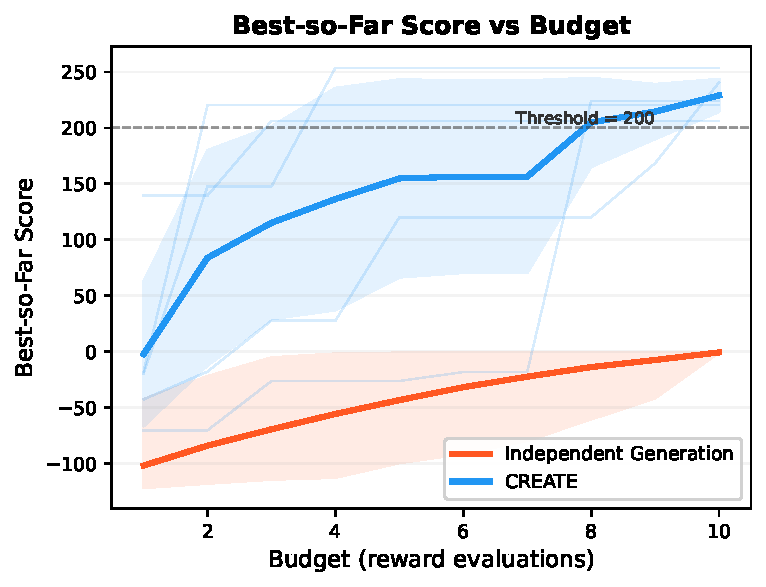
\includegraphics[width=\columnwidth]{performance_curve.pdf}\\[-2pt]
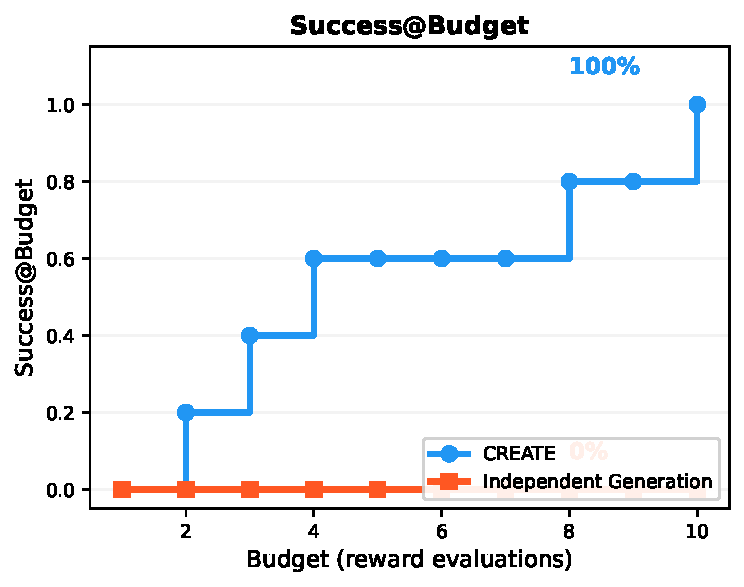
\includegraphics[width=0.485\columnwidth]{success_by_budget.pdf}\hfill
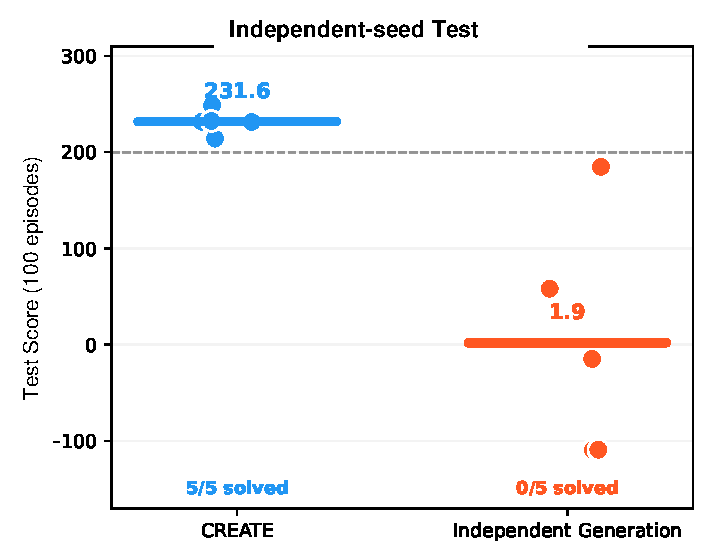
\includegraphics[width=0.485\columnwidth]{independent_test_scatter.pdf}
\caption{Budgeted reward search on LunarLander. Shading in (a)
spans the five runs; (b) reports the fraction whose incumbent crosses 200; (c)
compares repair and independent-test scores for selected rewards. Every point
comes from archived native-reward evaluations.}
\label{fig:performance}
\end{figure}

The repair histories also reveal two complementary modes of improvement.
L1 edits preserve a component's mathematical form and correct its scale; for
example, reducing an over-weighted progress term turns one LunarLander lineage
from $-29.48$ to $120.02$. L2 edits change the reward geometry when scaling
cannot help: replacing an unreachable multiplicative landing term with
independently reachable partial-credit factors takes another lineage from
$-17.90$ to $220.24$. CREATE is therefore not merely climbing a score curve.
It first decides whether the defect is parametric or structural, then changes
one component at the corresponding level.

\begin{table}[H]
\caption{Continuous-control transfer on BipedalWalker. ``Crossing'' is the
first reward that reaches the native threshold of 300.}
\label{tab:bipedal}
\centering
\scriptsize
\setlength{\tabcolsep}{4.0pt}
\begin{tabular}{ccccc}
\toprule
Seed & Initial & Crossing & Gain & Evaluations \\
\midrule
0 & 270.71 & 318.32 & $+47.60$ & 2 \\
1 & 280.50 & 313.46 & $+32.96$ & 2 \\
2 & 272.07 & 307.92 & $+35.85$ & 2 \\
3 & 289.99 & 311.12 & $+21.14$ & 2 \\
4 & 103.03 & 304.92 & $+201.90$ & 3 \\
\bottomrule
\end{tabular}
\end{table}

Table~\ref{tab:bipedal} tests whether the same repair logic transfers from
discrete actions to continuous control. Four initial rewards are already close
to threshold, so their gains show conservative refinement. The difficult seed
provides the stronger mechanism test: forward progress plus stability reaches
only 103.03, the first bounded refinement raises it to 264.39, and adding an
energy-use component crosses 300. Together, the trajectories show that CREATE
can preserve a useful reward skeleton while supplying a missing control
signal.

\subsection{Mechanism Ablations}
Figure~\ref{fig:ablation} separates selected-score quality from success
reliability.
Coarse feedback succeeds in 2/5 searches, showing that iterative editing alone
can work but is unreliable without component localization. Unconstrained
revision succeeds in 0/5 despite receiving structured evidence: observation
quality is insufficient when one action can rewrite several mechanisms at
once. CREATE achieves all five successes in 27 policy trainings, compared
with the fixed budget of 50 trainings used by independent generation.

\begin{figure}[H]
\centering
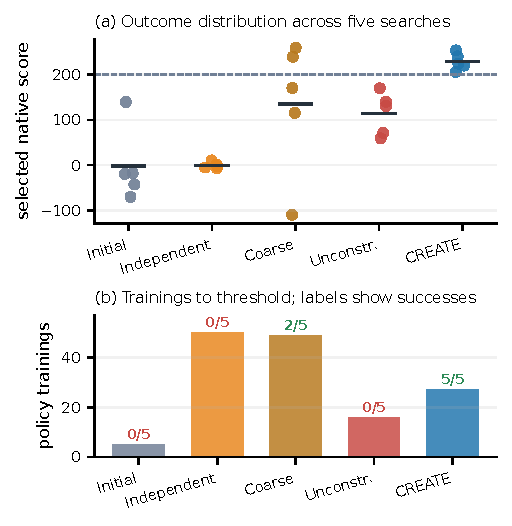
\includegraphics[width=\columnwidth]{ablation.pdf}
\caption{LunarLander mechanism ablations. Short horizontal marks in (a) are
five-run means. Panel (b) reproduces the archived realized-count view; its
ablation counts are descriptive rather than an efficiency comparison because
the corresponding iteration traces are incomplete.}
\label{fig:ablation}
\end{figure}

Independent candidates are parallelizable, whereas CREATE edits are
sequential. Hence, 27 versus 50 is a time-to-success
environment-interaction comparison, not a wall-clock claim. The independent
baseline also uses a simpler initialization prompt, and the combined
Unconstrained ablation does not separately identify edit hierarchy from edit
scope. We do not compare realized training counts for the two ablations
because their archived iteration traces are not complete and therefore do not
support a commensurate efficiency claim.

\subsection{Evidence-Guided Repair Case Study}
Figure~\ref{fig:case} follows LunarLander seed 0. Aggregate score alone looks
erratic. Component evidence reveals why. At iteration 7,
\texttt{approach\_shaping} is the only approach term to activate, yet the policy
terminates early in 19/20 episodes and never activates the touchdown or
stable-landing terms. The stored diagnosis predicts that a delta-distance
signal is too noisy and proposes an L2 replacement with a state-based
\texttt{landing\_proximity} term. The next run crosses the threshold and makes
landing-specific terms observable.

The trace ends at iteration 8, the first threshold crossing, and the best
archive returns that reward. Its record forms a checkable five-link chain. The
measured evidence is a score of $-388.67$, a
mean episode length of 109.5, 19/20 early terminals, and inactive landing
events. The diagnosis attributes these symptoms to a weak, noisy delta
approach signal. The L2 action replaces only that component with gated,
state-based landing proximity. Before training, the record predicts longer
episodes, reachable landing terms, and a higher native score. The next run
then reaches 224.21, with landing proximity active on nearly every step and
touchdown and stable-landing terms becoming observable. Because both the
prediction and the counter-risk were stored before the outcome, the trace can
be audited without relying on a post hoc narrative.

\begin{figure}[H]
\centering
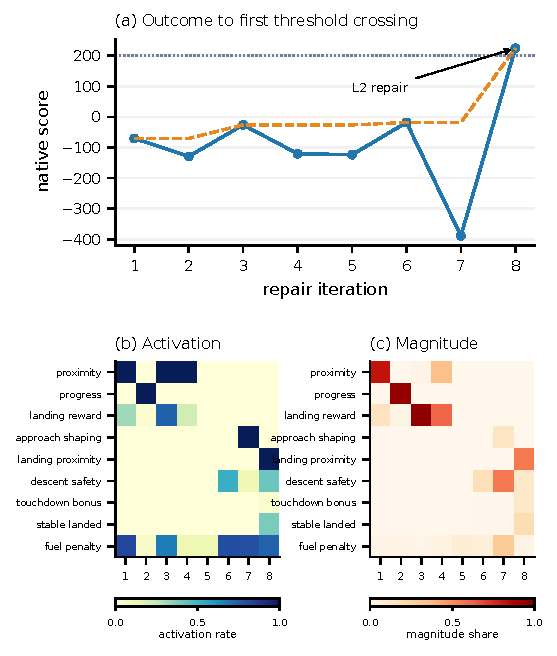
\includegraphics[width=\columnwidth]{repair_case.pdf}
\caption{One auditable repair. (a) Raw native scores are
shown only through the first threshold crossing. (b)--(c) show which named
reward components activate and dominate each training run; their separate
color bars encode activation rate and magnitude share, respectively. Missing
cells denote absent or inactive components, so interpretation also uses the
archived reward source and episode outcomes.}
\label{fig:case}
\end{figure}

\subsection{Data Provenance and Reporting Scope}
Every score in Figs.~\ref{fig:performance}, \ref{fig:ablation}, and
\ref{fig:case} comes from archived native-evaluation records. Each lineage also
stores reward source, episode outcomes, component statistics, diagnosis, and
edit level, so the figures are reproducible. TensorBoard verifies PPO budgets;
cross-candidate comparisons use the common native evaluator in
Eq.~\eqref{eq:native}, since shaped returns have candidate-specific scales.

The independent-seed test addresses selection on fixed repair seeds, not new
dynamics or task shifts. BipedalWalker verifies continuous actions, but four
initial rewards are close to threshold; seed 4 is therefore the stronger
transfer example, while LunarLander provides the cleaner mechanism ablations.

\section{Discussion and Conclusion}
CREATE supports a narrow claim: a failed policy-training run can guide repair
of the reward that produced it. Component statistics localize the defect,
native evaluation prevents self-grading, bounded actions preserve attribution,
and the archive protects a successful incumbent.

Evidence remains limited to PPO, two benchmarks, and five searches per task.
Prompt-matched baselines, factorized edit ablations, more RL algorithms, and
broader tasks remain necessary. Within this scope, CREATE turns training
failure into a structured observation and repairs every tested lineage to its
task threshold.

\enlargethispage{5\baselineskip}
\fontsize{6.7}{7.1}\selectfont
\begin{thebibliography}{00}
\setlength{\itemsep}{-1.2pt}
\setlength{\parskip}{0pt}
\bibitem{sutton2018rl}
R. S. Sutton and A. G. Barto, \emph{Reinforcement Learning: An Introduction},
2nd ed. Cambridge, MA, USA: MIT Press, 2018.
\bibitem{ng1999policy}
A. Y. Ng, D. Harada, and S. Russell, ``Policy invariance under reward
transformations: Theory and application to reward shaping,'' in \emph{Proc.
ICML}, 1999, pp. 278--287.
\bibitem{hadfield2017inverse}
D. Hadfield-Menell, S. Milli, P. Abbeel, S. Russell, and A. Dragan, ``Inverse
reward design,'' in \emph{Advances in Neural Information Processing Systems},
vol. 30, 2017.
\bibitem{language2rewards}
W. Yu \emph{et al.}, ``Language to rewards for robotic skill synthesis,'' in
\emph{Proc. Conf. Robot Learning}, 2023, pp. 374--404.
\bibitem{text2reward}
T. Xie \emph{et al.}, ``Text2Reward: Reward shaping with language models for
reinforcement learning,'' in \emph{Proc. ICLR}, 2024.
\bibitem{eureka}
Y. J. Ma \emph{et al.}, ``Eureka: Human-level reward design via coding large
language models,'' in \emph{Proc. ICLR}, 2024.
\bibitem{card}
H. Sun, Y. Wu, H. Luo, J. Gu, and W. Xu, ``CARD: A large language model-driven
reward design framework via dynamic feedback for reinforcement learning,''
\emph{Knowledge-Based Systems}, vol. 326, p. 114065, 2025.
\bibitem{revolve}
R. Hazra, R. Moraes, S. Dasgupta, and J. Pajarinen, ``REvolve: Reward evolution
with large language models using human feedback,'' in \emph{Proc. ICLR}, 2025.
\bibitem{rfagent}
N. Gao, X. Zhang, X. Jiang, M. You, M. Zhang, and Y. Deng, ``RF-Agent:
Automated reward function design via language agent tree search,'' in
\emph{Advances in Neural Information Processing Systems}, vol. 38, 2025.
\bibitem{react}
S. Yao, J. Zhao, D. Yu, N. Du, I. Shafran, K. Narasimhan, and Y. Cao,
``ReAct: Synergizing reasoning and acting in language models,'' in
\emph{Proc. ICLR}, 2023.
\bibitem{reflexion}
N. Shinn, F. Cassano, E. Berman, A. Gopinath, K. Narasimhan, and S. Yao,
``Reflexion: Language agents with verbal reinforcement learning,'' in
\emph{Advances in Neural Information Processing Systems}, vol. 36, 2023.
\bibitem{voyager}
G. Wang, Y. Xie, Y. Jiang, A. Mandlekar, C. Xiao, Y. Zhu, L. Fan, and A.
Anandkumar, ``Voyager: An open-ended embodied agent with large language
models,'' \emph{arXiv preprint arXiv:2305.16291}, 2023.
\bibitem{wang2026diagnostic}
Y. Wang, Y. Tang, B. Liu, X. Liu, and D. Shang, ``When LLM reward design
fails: Diagnostic-driven refinement for sparse structured RL,'' \emph{arXiv
preprint arXiv:2605.28918}, 2026.
\bibitem{ppo}
J. Schulman, F. Wolski, P. Dhariwal, A. Radford, and O. Klimov, ``Proximal
policy optimization algorithms,'' \emph{arXiv preprint arXiv:1707.06347}, 2017.
\bibitem{sb3}
A. Raffin \emph{et al.}, ``Stable-Baselines3: Reliable reinforcement learning
implementations,'' \emph{J. Mach. Learn. Res.}, vol. 22, no. 268, pp. 1--8,
2021.
\end{thebibliography}
\end{document}
